\chapter{Results}

\section{Using the server/client solution with a mockup of the network}


The client\_shell is designed to be easy to use.
We start by launching the client\_shell. One short session with the client\_shell may look like this:


\begin{figure}[H]
\begin{center}
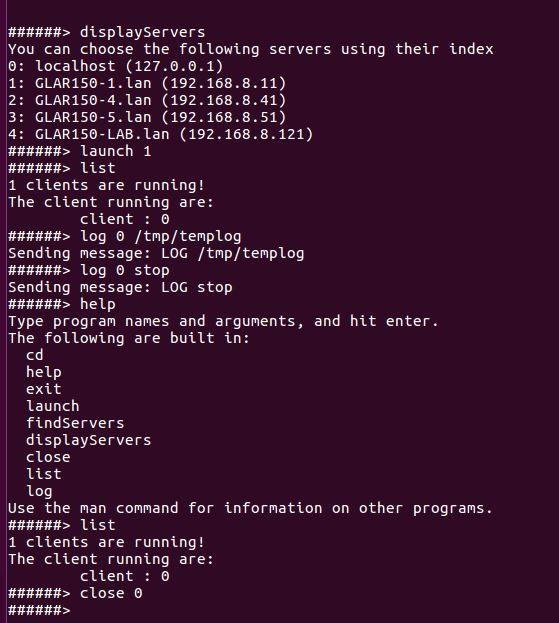
\includegraphics[width=0.7\textwidth]{image/clientshell.jpg}%
\caption{Using the client\_shell}%
\label{figure:clientshell}%-
\end{center}
\end{figure}

On the above figure, we can see how to use the client\_shell with an example.
I am launching a client for the server 1. I am telling to log the data in a file called /tmp/templog. After waiting a moment, I asked it to stop logging. At the end of the session, I am telling the client to stop the communication.


When using the launch command, a new terminal will open. This terminal is the client. It will connect to the server, print data and listen for orders from the user.

\begin{figure}[H]
\begin{center}
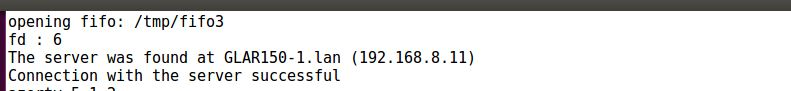
\includegraphics[width=0.7\textwidth]{image/clientinit.jpg}%
\caption{The client is connection to the server}%
\label{figure:clientint}%-
\end{center}

\end{figure}\begin{figure}[H]
\begin{center}
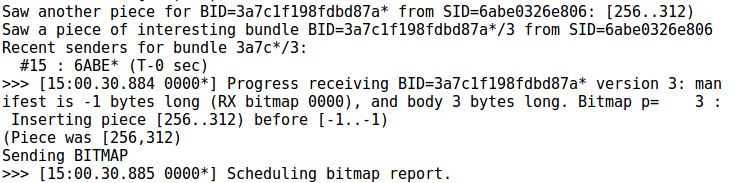
\includegraphics[width=0.7\textwidth]{image/clientcomm.jpg}%
\caption{The client is receiving data}%
\label{figure:clientcomm}%-
\end{center}

\end{figure}\begin{figure}[H]
\begin{center}
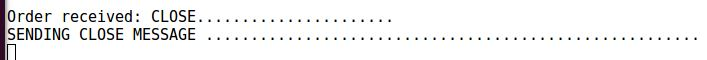
\includegraphics[width=0.7\textwidth]{image/closeclient.jpg}%
\caption{Closing the client}%
\label{figure:closeclient}%-
\end{center}
\end{figure}

The three figures above present the 3 types of action the client is executing. On the first figure, the client check if the server exists and establishes the communication with the server. On the second figure, the client is printing data received from the server. On the last figure, the client received the order "STOP" from the client\_shell (command close) and tell the server to stop before closing itself.

All these tests were made using a mockup version of the network. The server was in the same room as the computer. However, the computer had to go through the main router to reach the server. 




\section{Monitoring the Wi-Fi}

Using the workaround solution, I was able to monitor the remote router. 

\begin{figure}[H]
\begin{center}
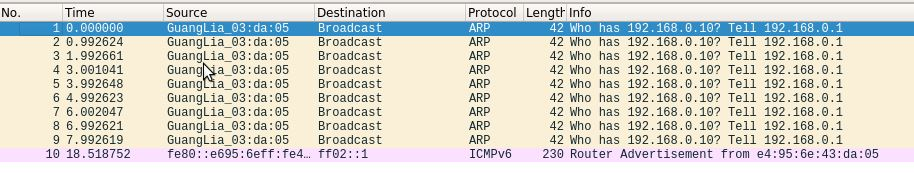
\includegraphics[width=\textwidth]{image/wireshark.jpg}%
\caption{Remote Wi-Fi analysis}%
\label{figure:wireshark}%-
\end{center}
\end{figure}

The figures show the wireshark running on the computer. The packets shown on the wireshark are packets on the LAN interface of the remote router.



\section{Remotely controlling the phone}

Currently, the remote phone control solution is not working with the small routers. As a proof of concept, it is working on a computer.
Here is the result I have using scrcpy:
\begin{figure}[H]
\begin{center}
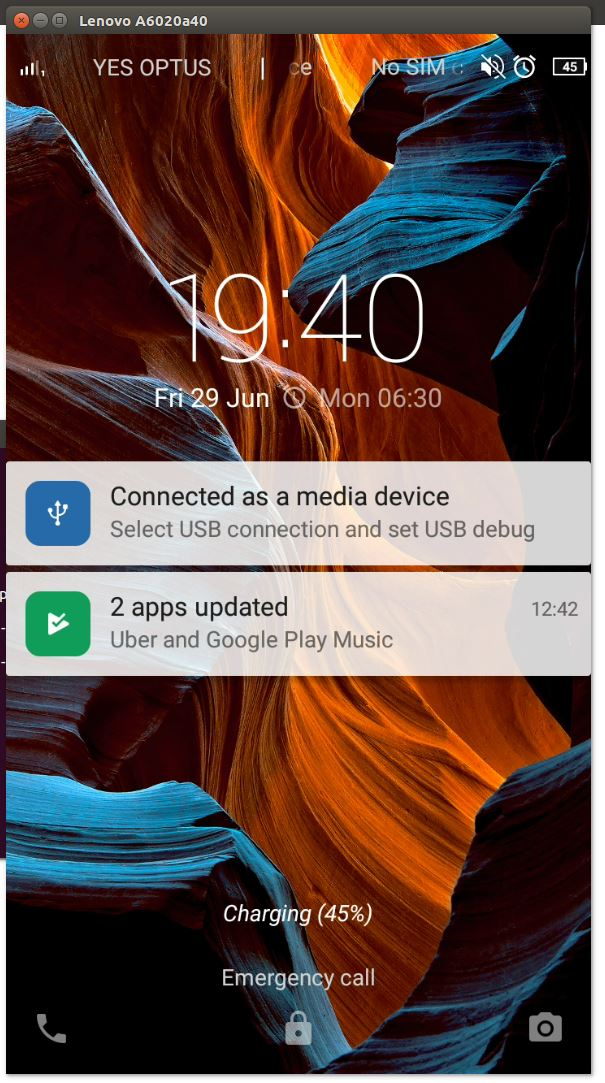
\includegraphics[width=0.3\textwidth]{image/phonecapture.jpg}%
\caption{Remote phone control}%
\label{figure:phone}%-
\end{center}
\end{figure}

On the computer, I was able to display the screen of my phone and access to everything on it. I had a full access to the phone. I could send sms or use applications from my computer.